In Section \ref{subsec:fgrPCA} \ac{PCA} was used used to show that three eigenvectors are sufficient to capture over 99\% of the variance in Bison's simulated Ris\o~ AN3 power ramp fission gas release time series. The variation is caused by perturbations in the fission gas release parameters although they are not explicit in the \ac{PCA} framework. The Dakota code is used to create the 100 time series in the previous section. In accordance with each parameter's uniform distribution described in Table \ref{table:fgr_params}, Dakota made 100 sets of perturbations to the parameters using the \ac{LHS} method. Each of the 100 samples was then propagated through Bison and a time series of fission gas release was output. \ac{PCA} was then performed on the covariance matrix of the 100 samples. Consequently, there is a clear mapping from a set of eight fission gas release parameters to a time series. More specifically, there is a mapping from the i$^{th}$ set of eight parameters $R^{i}$ to the three expansion coefficients $\lbrace p_{i1}, p_{i2}, p_{i3} \rbrace$ that are capable of reproducing the time series, as described in Eq. \ref{eq:pcaExpCoeffs}. In order to predict new time series for a set of fission gas release parameters not in the set used to derive the three principal components this mapping must be generated. Kriging is used achieve the mapping.  

To start, using the Kriging description in Section \ref{sec:kriging} a surrogate is constructed for each of the expansion coefficients related to the three principal components responsible for over 99\% of the variance. Each of these surrogates $\hat{p}_{ij}$ for $j\in\left(1,2,3\right)$ accepts a set of fission gas release parameters and outputs a scalar expansion coefficient for the principal component $X_j$. In accordance with Eq. \ref{eq:pcaExpCoeffs} the predicted fission gas release time series is,
\begin{equation}
\label{eq:predicted_mean_fgr_ts}
 \hat{\mathcal{F}}^{i}(R^i) = \hat{p}_{i1}\left(R^i\right) X_1 + \hat{p}_{i2}\left(R^i\right) X_2 + \hat{p}_{i3}\left(R^i\right) X_3 + \mu  
\end{equation}
where $\mu$ is the mean release time series of the 100 simulations. Since Kriging surrogates return an uncertainty $\sigma_{\hat{p}_{ij}}$ along with a predicted scalar value, an uncertainty band can be derived for the time series in Eq. \ref{eq:predicted_mean_fgr_ts}.
\begin{equation}
\label{eq:predicted_std_fgr_ts}
 \sigma_{ \hat{\mathcal{F}}^i }^2 = \sigma_{\hat{p}_{i1}}^2 X_1^2 + \sigma_{\hat{p}_{i2}}^2 X_2^2 + \sigma_{\hat{p}_{i3}}^2 X_3^2 
\end{equation}
The shape of the uncertainty vector output by Eq. \ref{eq:predicted_std_fgr_ts} is equal to the number of time-steps utilized in the principal components. 

\subsubsection{Cross Validation}
\label{subsec:cross_validation}

With a Kriging formulation for predicting Ris\o~ AN3 power ramp fission gas release time series for any set of Bison fission gas release parameters in place, it is necessary to test the formulation. In other words, it's necessary to investigate the error in the formulation's predictions. If the Kriging surrogates can accurately predict their respective \ac{PCA} expansion coefficients then the formulation will be able to accurately predict gas release time series since Eq. \ref{eq:predicted_mean_fgr_ts} is just a linear combination of the predictions. To this end, a test set of 100 independent Bison simulations of the Ris\o~ AN3 power ramp were obtained. The simulations in the test set are completely isolated from those in the training set and not used in calculating the Kriging surrogates nor the principal components. There are several common approaches to judging the validity of a predictive model as described in \cite{Jones_Schonlau}. With training and test sets available at disposal are true expansion coefficient values, predicted values, and uncertainties in the predicted values. Using these components the standardized cross-validated residual is defined as,
\begin{equation}
\label{eq:stnd_xval_residual}
 \frac{ p_{ij} - \hat{p}_{ij} }{ \sigma_{\hat{p}_{ij}} } . 
\end{equation}  
The standardized cross-validated residuals for all three Kriging surrogates' predictions on the test set are shown in Fig. \ref{fig:xval_3sig_bands}. Note the Kriging models used to predict the expansion coefficients are built on 100 samples analyzed previously in Sec. \ref{subsec:fgrPCA}.  
\begin{figure}
\caption{\label{fig:xval_3sig_bands}
Cross validation of Kriging predictions for \ac{PCA} expansion coefficients using 3$\sigma$ band approach.}
 \begin{center}
  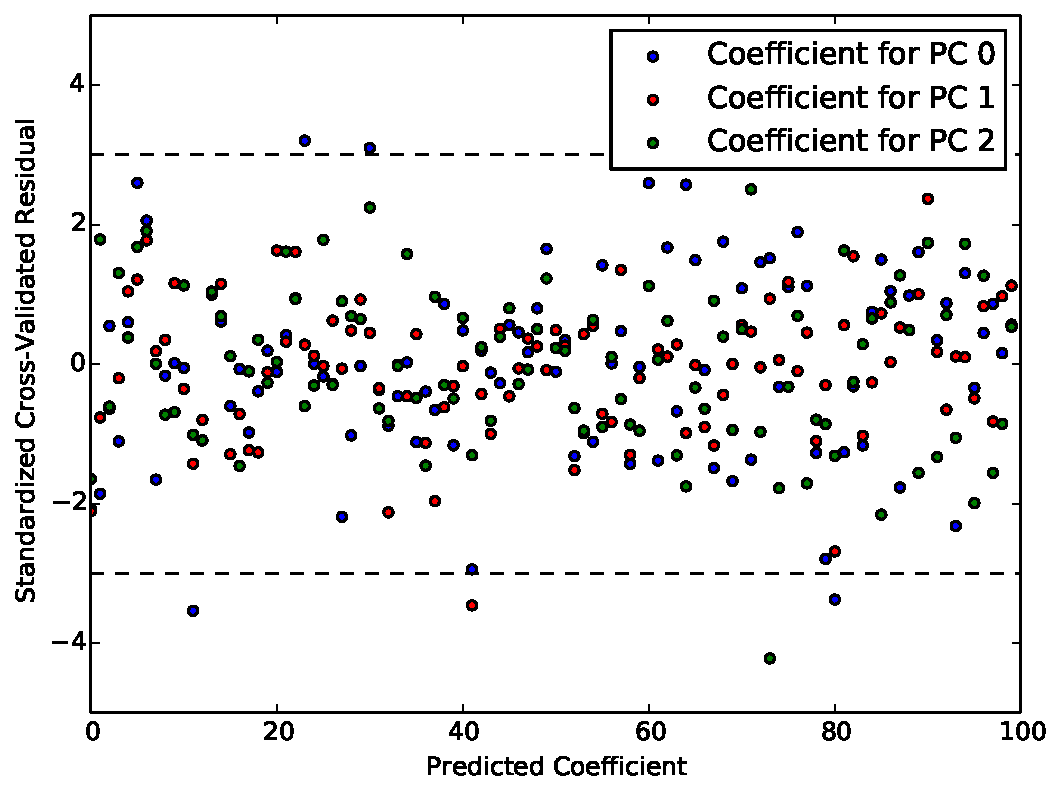
\includegraphics[scale=.75]{./Chapter4/xval_3sig_band.pdf}
 \end{center}
\end{figure}
Each point represents the number of standard deviations the true expansion coefficient is to the predicted coefficient. Some 99.7\% of points are expected to lie within the band $\left[-3, +3\right]$. Indeed, of the 300 points appearing in Fig. \ref{fig:xval_3sig_bands} some six lie outside the bands, which is a first indication that the predictive model has merit.  

In the second cross validation approach, the predicted values are plotted directly against the true values as shown in Fig. \ref{fig:xval_45degree}. Ideally, all points would lie on the 45$^{\circ}$ line, which would indicate that predictions perfectly match the true expansion coefficient values. The plots in Fig. \ref{fig:xval_45degree} show that the predicted values do generally approach this trend despite the presence of some noise. For predictions of each expansion coefficient in Fig. \ref{fig:xval_45degree} the results are plotted when 20, 60, and 100 random samples from the test set are utilized. Of course, less noise is present as the number of samples used to build the surrogates increase.  
\begin{figure}
\caption{\label{fig:xval_45degree}
Cross validation of Kriging predictions for \ac{PCA} expansion coefficients using 45$^\circ$ approach.}
 \begin{center}
  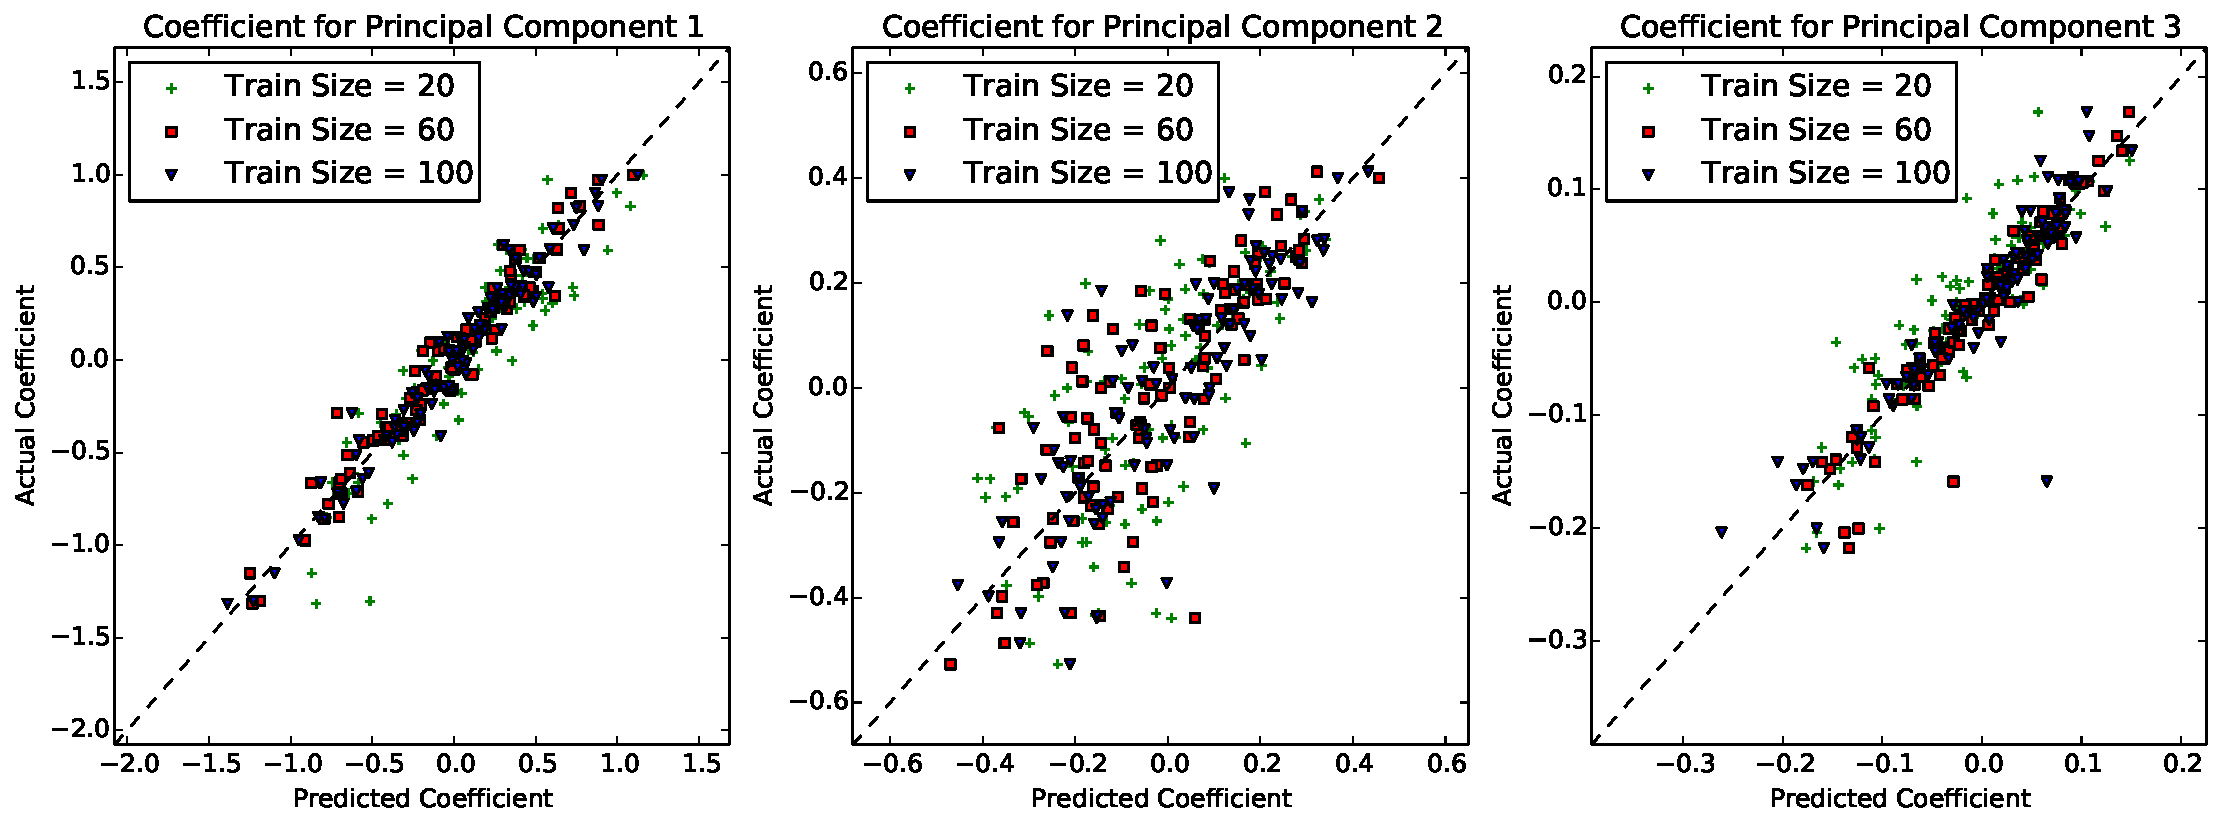
\includegraphics[scale=.4]{./Chapter4/xval_45degree.pdf}
 \end{center}
\end{figure}
Surprisingly, regardless of the training set size, predictions for the first principal component expansion coefficient are of the highest quality followed by the predictions for the expansion coefficients of the third principal component. It is most important to accurately predict expansion coefficients for the top principal components since they explain the most variance. Accurate prediction of lower principal components offers diminishing returns. Both inverse and logarithmic transforms were applied to the data as suggested in \cite{Jones_Schonlau} although no noticeable improvement was observed in prediction accuracy.   

\subsection{Calibration}
\label{\subsec:calibration}

Now that the predictive accuracy of the individual Kriging surrogates for each expansion coefficient have been cross validated it is time to investigate how well the surrogates can perform collectively in predicting Ris\o~AN3 power ramp fission gas release time series. To determine the error between predicted time series the \ac{RMSE} is used as a cost function. Recall that before any two time series are compared each is segmented into 150 identical locations. The objective of calibration is to find a set of fission gas release parameters $R^i$ such that when they are input into Eq. \ref{eq:predicted_mean_fgr_ts} the \ac{RMSE} is minimized. 

Ideally, the landscape of possible \ac{RMSE} values is such that a clear global minimum exists. In this case, an algorithm such as \ac{EGO} can be used to find the minimal value and its corresponding parameter set \cite{Jones_Schonlau}. \ac{EGO} couples a computer model's surrogate prediction and uncertainty with the computer model itself in an iterative optimization process.  At each iteration \ac{EGO} estimates the parameter space location that is most likely to contain a \ac{RMSE} value smaller than the current minimum. The true computer model is then evaluated at this point and therefore, the minimization procedure can be potentially expensive. However, if it is known a priori that the \ac{RMSE} landscape is for example, convex then \ac{EGO} should be strongly considered. Unfortunately, there is usually no way to tell a priori the shape of a landscape for most expensive engineering codes such as Bison. Due to the non-linearities inherent in such codes the landscape is often fairly "flat". A flat landscape can result when some parameters are insignificant and thus, many values of these parameters will result in similar cost function values. Also, a flat landscape can result if the minimization problem is non-unique, meaning many combinations of parameters can yield the same, or nearly the same, optimal values for the \ac{RMSE}. Often times, these two issues may be interrelated and both will tremendously complicate the global optimizer search. Indeed, if \ac{EGO} is used many expensive computer code evaluations will be wasted. A local optimization algorithm should be utilized if a flat landscape is suspected.  

In order to decide which time of minimization algorithm to apply to the problem in-hand Sobol indices are calculated using the surrogate model. 
% Morris plot 

       






   

